\section{Introduction} \label{INTRO}
A very basic understanding of rendering in the traditional sense is assumed. Rasterization, the basics of the SIMT execution model and general graphics terms like global illumination are all assumed. In this section we will first provide some foundational knowledge on the topic of ray tracing (Section \ref{INTRO:tracing}). Then we describe the context in which these techniques are implemented at \href{https://traverseresearch.nl/}{Traverse Research} (Section \ref{INTRO:traverse}). Afterwards we explore some of the background research in volume rendering (Section \ref{INTRO:volumes}), how to accelerate it (Section \ref{INTRO:volume_acceleration}) and the current state of the art (Section \ref{INTRO:VDB}). These should provide enough background information to be able to understand this research.

\subsection{Rendering in games} \label{}
\subsubsection{Rasterization} 
\subsubsection{Ray and path tracing} \label{INTRO:tracing}
Rasterization is the rendering technique which has been the industry standard for at least the past 20 years. It involves processing every triangle in the scene. Then, using a set of transforms, these triangles are draw on the screen. Graphics hardware has been built around this pipeline, but it does have limitations. For example, reflections can not show off-screen objects without sophisticated (and often slow) tricks. Ray tracing is an entirely different technique which shoots a ray for every pixel, finds the triangle which intersects that ray, and then shades it. This has the benefit of no longer needing to process every triangle individually, and instead can search for an intersecting triangle quickly. A high level overview of said algorithms can be seen below:

\begin{tabular}{|l|l|}
    \hline
    Technique & Overview\\
    \hline
    Rasterization & \makecell[l]{For each triangle:\\ \quad For each pixel it covers:\\ \qquad Shade} \\
    \hline
    Ray tracing & \makecell[l]{For each pixel:\\\quad Find triangle it intersects:\\ \qquad Shade} \\
    \hline
\end{tabular}

\begin{figure}[H]
    \centering
    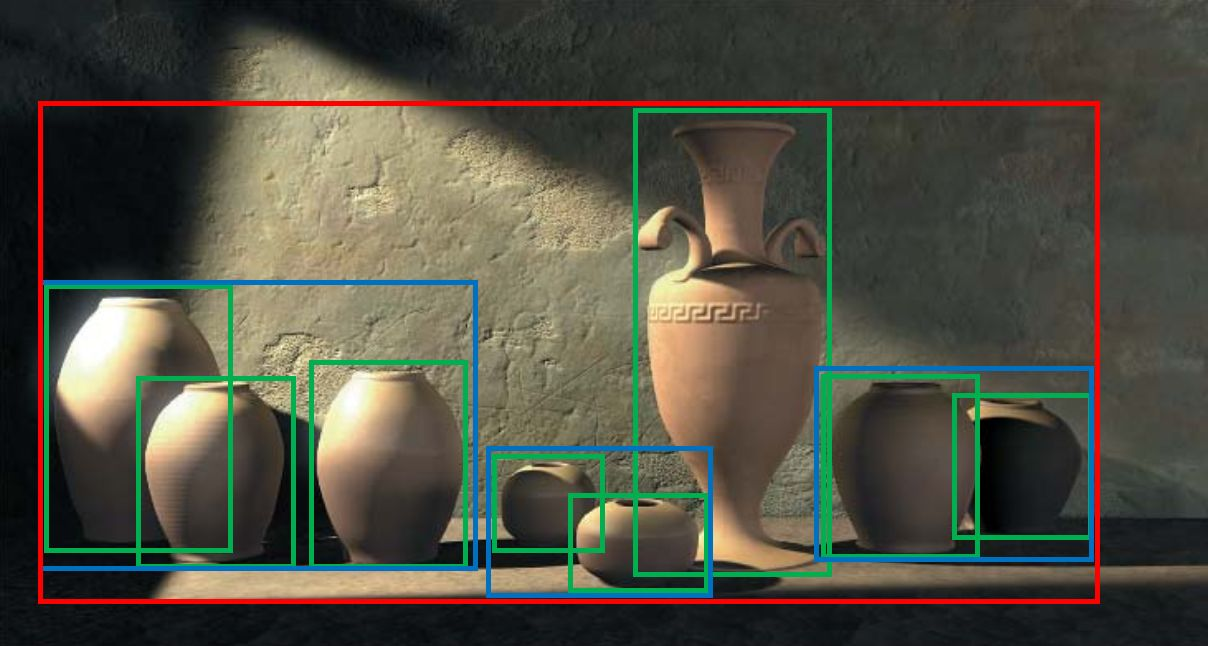
\includegraphics[width=0.9\linewidth]{figures/bvh.jpg}
    \caption{A bounding volume hierarchy where the red bounding box encapsulates all objects. Then a step lower in the hierarchy we see the blue bounding boxes which encapsulate groups of objects. And the leaves, indicated by the green bounding boxes, contain the primitives. These structures are stored in a tree like structure and can, theoretically, have infinite depth or width. Finding the intersection between a ray and the bounding volume hierarchy can be done in $O(\log n)$ time on average, where n is the number of primitives. \cite{BVHJacco}}
    \label{fig:bvh}
\end{figure}

Although ray tracing has been theorized by many to be the replacement of classic rasterization methods, we have only recently seen it being applied to games after NVIDIA released its RTX graphics cards. Additionally, we see that all AAA games currently still depend on the rasterizer and only use ray tracing to enhance their graphics either by adding realistic (1) diffuse indirect light, which is often mislabeled as GI, (2) shadows, (3) reflections, (4) ambient occlusion or a combination of these four\cite{NVIDIARTX}. 

Path tracing is a specific algorithm which uses ray tracing to calculate physically accurate images by trying to solve the rendering equation \cite{kajiya1986rendering}. It does this by recursively performing a Monte Carlo experiment over the integral in the rendering equation for every pixel. This results in a realistic image once converged. However, for the longest time this has been too slow to run in real-time on commodity hardware. Fortunately, there have been some major advances in (1) sampling techniques as described in \cite{lin2022generalized} and (2) filtering techniques as described in \cite{yang2020survey}. Along with the advent of better GPU hardware, it might make real-time path tracing a reality for upcoming AAA games. 

Generally, path tracing involves multiple steps to achieve real time performance \cite{laine2013megakernels}, (1) ray generation, (2) ray extension, (3) shading and (4) shadow ray extension. This pipeline is executed for every pixel on screen, so for a standard 1080p monitor that would be $1920*1080=2.073.600$ rays. Step 1 is executed once at the start, and then the latter three steps are done repeatedly to simulate realistic light transport through the scene. The main task of steps 2 and 4 is to find an intersections with the scene geometry. This can be done by individually performing intersection tests with every triangle in the scene with a time complexity of $O(n)$, where $n$ is the number of triangles. However, this linear scaling is prohibitive when the complexity of models increases. So to fix this problem, bounding volume hierarchies (BVH as seen in Figure \ref{fig:bvh}) are used to accelerate these intersection tests. This is done by creating a traversable tree with triangles at the leaf nodes, which reduces the average traversal time to  $O(\log n)$. To allow instanced rendering without drastically increasing the triangle count of the scene or increasing build times, a top level acceleration structure (TLAS) is created over a bottom level acceleration structure (BLAS). Here the TLAS contains pointers to multiple BLAS's which contain the actual model data \cite{VulkanAccelerationStructures}. 

\subsection{Volume rendering} \label{INTRO:volumes}
In this project volume data represents clouds, explosions, fire and sand/dust storms. This means that we are not just interested in finding the boundary of a volume, but also in the contents of the volume. We may have varying densities or even different materials within one volume. For example, a flame which emits light surrounded by smoke, where the outer edge of this smoke is so sparse that it is almost completely transparent. When shading these kinds of materials there are three main things which can happen: (1) The ray is absorbed, meaning that no light transport will be rendered. When this happens, the light energy is converted into another energy form like heat. (2) The ray is traversed through or bounces off the particle. This will change the direction of the ray and potentially change the ray payload, for example when a blue particle is hit, the ray is modified to only return the blue color if a light is hit. (3) The ray hits an emissive particle. Meaning that light transport will be rendered, and the ray will not continue.

Ray tracing these kinds of volumes is very different from normal ray tracing, as they require completely different methods. Normally there is a set of surfaces which define a scene. To render these scenes, BVH's are used to find an intersection between a ray and the scene as described in Section \ref{INTRO:tracing}. For volume rendering we don't have these concrete surfaces but instead have volumes with implicit particles, like dust or water droplets from a cloud. To render these volumes we somehow have to find where we hit such a particle and evaluate its shading function. We do not simulate these particles individually but describe volumes of the scene using densities, which are discretized into small volumetric pixels (voxels). When traversing such a volume we calculate how far we can traverse through these densities before we are likely to hit a particle. Then we take the step, evaluate the shading function and calculate how long our next step can be. This process is called ray marching \cite{RenderingWithTwoTriangles}. For homogeneous volumes (with a uniform density) these step sizes will always be the same, but for heterogeneous volumes they might not. In the heterogeneous case we calculate the longest possible step we could take through the most dense voxel in our scene and use that to make sure we do not overshoot and miss any dense voxels. This method quickly becomes prohibitively expansive when a single voxel has a high density. A solution would be to take steps proportional to the highest local density, for example the highest density of the $8^3$ nearest voxels. This way we can take step sizes which are proportional to the densities which we are more likely to traverse, instead of crippling the performance for every ray because of a single voxel \cite{kutz2017spectral}.

\begin{figure}[H]
    \centering
    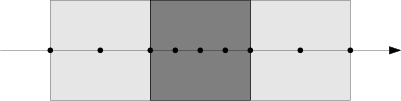
\includegraphics[width=0.9\linewidth]{figures/sample_step_size.png}
    \caption{A ray traversing through a heterogeneous volume, where dots represent the location of shading evaluations. As can be seen, the more dense the volume (darker) the shorter the steps are.}
    \label{fig:sample_step_size}
\end{figure}

\subsection{Traverse Research} \label{INTRO:traverse}
\href{https://traverseresearch.nl/}{Traverse Research} is a company which does state-of-the-art research in graphics, and more specifically ray tracing. Their current in-house hybrid rendering framework "Breda" includes many features which are expected from a modern renderer. However, volume rendering is still largely unexplored. Breda can compile for either a Vulkan or a DirectX 12 backend to make use of the latest ray tracing features. Along with that, some advanced rendering techniques are used. Most notably bindless rendering\cite{BindlessRenderingSetup} and render graphs\cite{RenderGraph101}. The former is a different way of interfacing with data on the GPU, while the latter simplifies GPU synchronization while optimizing dispatch ordering based on read and write dependencies of different pieces of data on the GPU. All of this is written in Rust and HLSL, which this project must adhere to. 

At \href{https://traverseresearch.nl/}{Traverse} there is another parallel project which involves volumetrics. That project focuses on shading as explained in Section \ref{INTRO:volumes}. Merging the shading with the result of this project should allow for physically based shading with fast volume traversal in order to perform real-time realistic volumetric rendering. The exact placement of this project inside the Breda framework can be seen in Figure \ref{fig:project_structure}.

\begin{figure}[H]
    \centering
    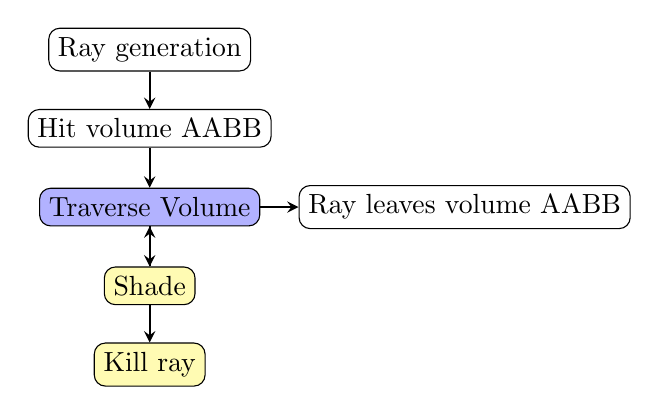
\begin{tikzpicture}[node distance=1cm]
    \tikzstyle{arrow} = [thick,->,>=stealth]
    \tikzstyle{done} = [rectangle, rounded corners, minimum width=1cm, minimum height=0.33cm,text centered, draw=black]
    \tikzstyle{this} = [rectangle, rounded corners, minimum width=1cm, minimum height=0.33cm,text centered, draw=black, fill=blue!30]
    \tikzstyle{other} = [rectangle, rounded corners, minimum width=1cm, minimum height=0.33cm,text centered, draw=black, fill=yellow!30]
    \node (start) [done] {Ray generation};
    \node (aabb) [done, below of=start] {Hit volume AABB};
    \node (trav) [this, below of=aabb] {Traverse Volume};
    \node (shade) [other, below of=trav] {Shade};
    \node (kill) [other, below of=shade] {Kill ray};
    \node (leaves) [done, right of=trav, xshift=3cm] {Ray leaves volume AABB};

    \draw [arrow] (start) -- (aabb);
    \draw [arrow] (aabb) -- (trav);
    \draw [arrow] (trav) -- (shade);
    \draw [arrow] (trav) -- (leaves);
    \draw [arrow] (shade) -- (trav);
    \draw [arrow] (shade) -- (kill);
    
    \end{tikzpicture}
    \caption{Flow diagram of the volume rendering project inside \href{https://traverseresearch.nl/}{Traverse}. The white boxes indicate parts of the pipeline which already exist inside the Breda framework. The blue box shows what this project will focus on, and the yellow boxes highlight what parts are happening in parallel with this project. As can be seen, when rays bounce inside a volume, they can repeatedly be shaded and continue traversal until they either leave the volume or are killed because they wont contribute any light to the scene.}
    \label{fig:project_structure}
\end{figure}

\subsection{Accelerating volume traversal} \label{INTRO:volume_acceleration}
Data structures for heterogeneous volumes have seen multiple forms trying to optimize ray marching performance, memory footprint, update speed and simplicity. As described in Section \ref{INTRO:volumes}, this project specifically targets heterogeneous volumes which often consist of gradients where outer voxels can have small non-zero values, instead of having opaque volume boundaries. This might alter the effectiveness of certain methods or require reducing the precision of our data in favor of traversal speed. For example, we could compress a set of voxels which have similar density values into a single larger voxel with the averaged density. This will make the data structure lossy but might significantly improve traversal speed or memory footprint. We will briefly go over some of the major volume data structures, below. 

\noindent\textbf{Flat 3D array:} The most basic structure (see Figure \ref{fig:dda_traversal}). Here, every value in the 3D array corresponds to a voxel. Indexing into this structure is fast and editing is trivial. However, there is no compression or empty space skipping. All rays might have to step through the entire volume one step at a time (which is often done using the Digital Differential Analyzer (DDA) algorithm \cite{amanatides1987fast}) which does not scale well to volumes with larger resolutions. Another problem with flat arrays is their memory requirement as it has cubic scaling with the resolution. However, small scale simulation software still often relies on this data structure as it is easy to implement, and in many cases simulations have to update each voxel anyway.

\begin{figure}[H]
    \centering
    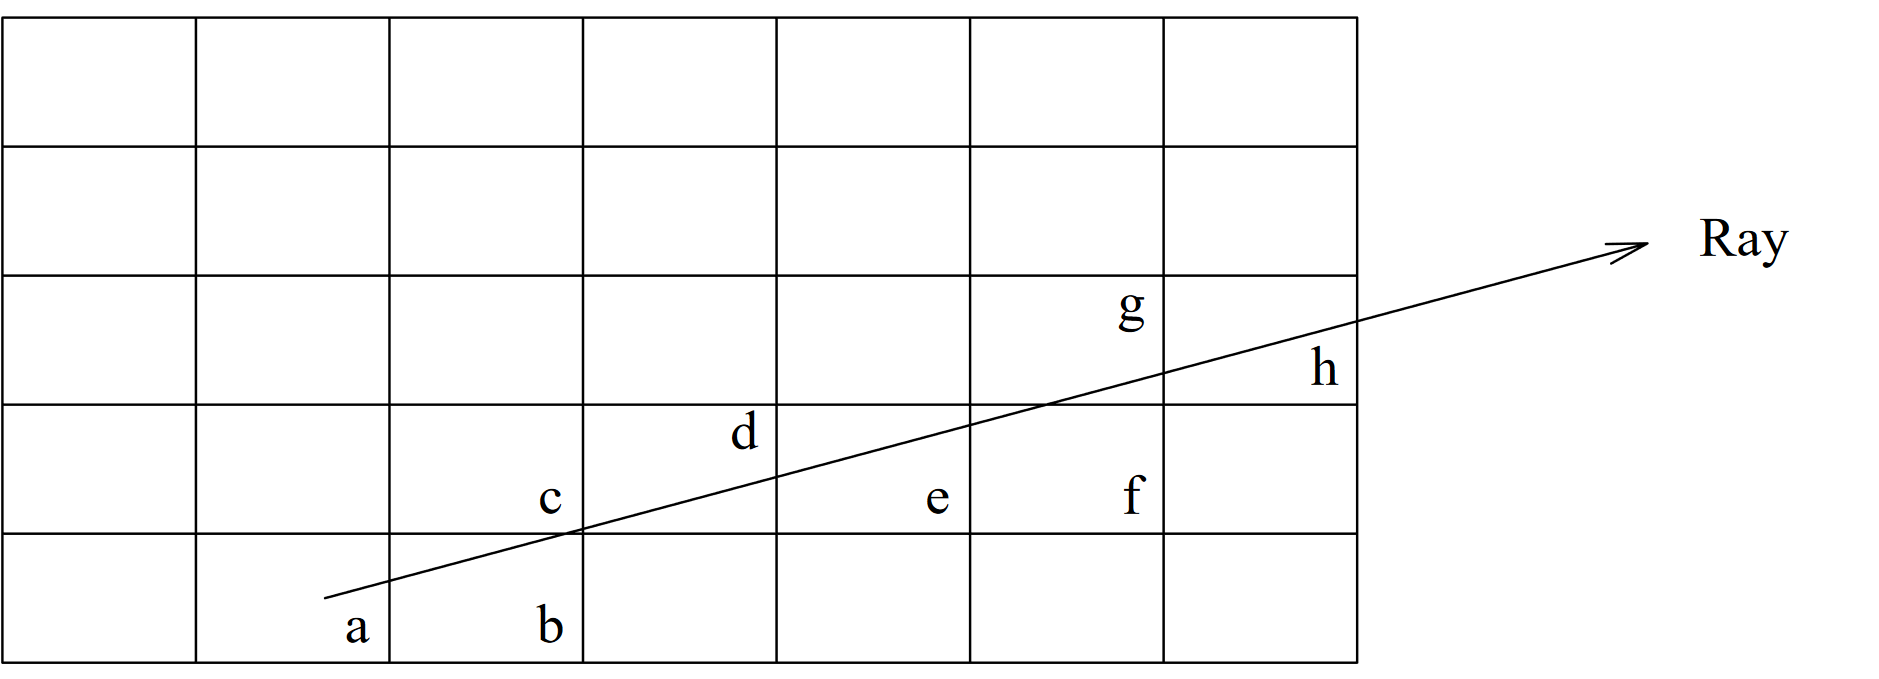
\includegraphics[width=0.9\linewidth]{figures/dda.png}
    \caption{DDA traversal through a flat grid. Step through every voxel that intersects the ray. \cite{amanatides1987fast}}
    \label{fig:dda_traversal}
\end{figure}

\noindent\textbf{Efficient Sparse Voxel Octrees (ESVO):} A solution to the memory problems was proposed by NVIDIA, by introducing sparsity to homogeneous volume data \cite{laine2010efficient}. The main contribution is a data structure which drastically reduces the memory footprint by not storing information about homogeneous areas. This memory reduction also yields a speedup when traversing the volume, as larger steps can be taken through homogeneous areas (see Figure \ref{fig:esvo}). Along with that, the structure will more easily fit in the different caches of the GPU. However, due to the nature of tree structures, the data access pattern is less coherent which negatively impacts ray marching performance. The paper also did not take any form of animation into account. So this data structure only really works on static scenes \cite{JohnLinPerfectEngine}. 

\begin{figure}[H]
    \centering
    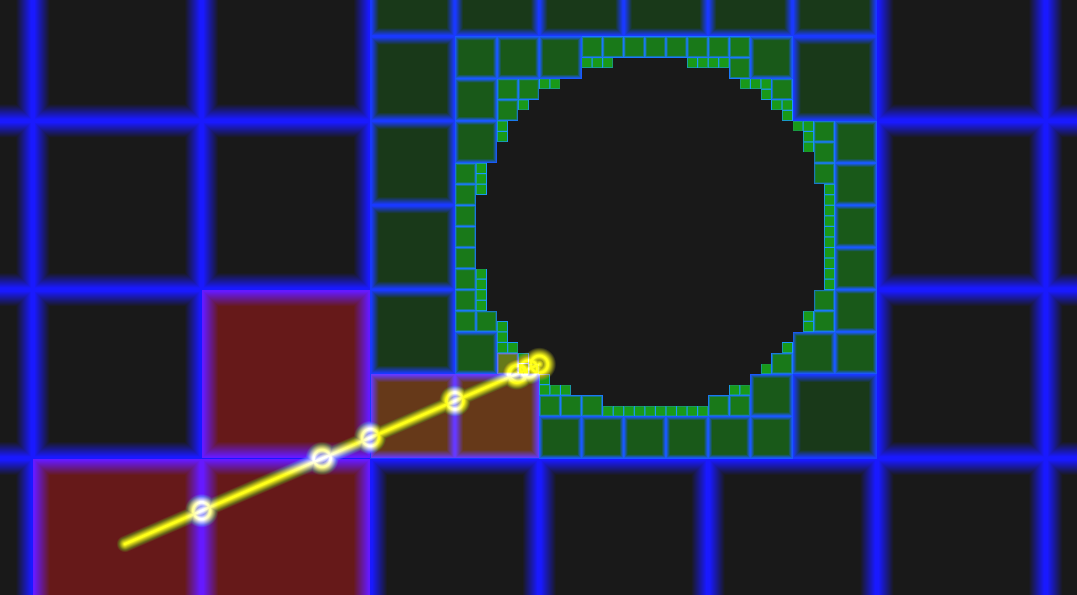
\includegraphics[width=0.9\linewidth]{figures/esvo_traversal.png}
    \caption{Hierarchical DDA traversal through a sparse voxel octree. The yellow line is our ray. The brighter green a cell is, the deeper our nodes in the octree are. We can see that nodes which are further away from the circle, can be stepped through with big steps, but as we approach the circle, our steps become smaller. Image obtained from Shadertoy.}
    \label{fig:esvo}
\end{figure}

\noindent\textbf{High Resolution Sparse Voxel DAGs (SVDAG):} A follow-up paper was released further improving the memory footprint optimization \cite{kampe2013high}. Here, the nodes of the octree can be reused for identical volumes, so one leaf can be the child of multiple nodes that share the same data (see Figure \ref{fig:DAG_node_deduplication}). The result is a significant reduction in memory usage over ESVO. Afterward, additional papers were written to, (1) further optimize the memory footprint by creating a lossy data structure which will slightly alter the volume data in an attempt to find more similar volumes \cite{van2020lossy} (LSVDAG). And (2) allow for real time editing of this data structure \cite{careil2020interactively} (HashDAG). 

\begin{figure}[H]
    \centering
    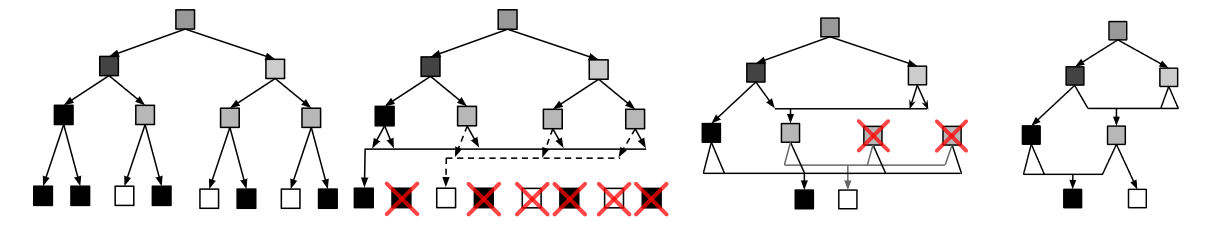
\includegraphics[width=0.9\linewidth]{figures/DAG_node_deduplication.png}
    \caption{Removal of identical nodes in all levels of a binary tree. In the SVDAG paper the same technique is applied to octrees. \cite{kampe2013high}}
    \label{fig:DAG_node_deduplication}
\end{figure}

\noindent\textbf{Brickmaps:} Later another paper was released which tried to maintain part of the memory benefits from octrees while also improving ray marching performance \cite{van2015real}. This was done by keeping the idea of a hierarchical structure, but limiting the tree depth to 2 layers (a top level grid, the brickmap and the bottom level bricks, as can be seen in Figure \ref{fig:brickmap}), which improves cache utilization. An additional benefit of reducing the depth of a data structure is the update time. When running a fluid simulation, which has to touch every leaf node in a tree, a shallower tree will take fewer steps when going down to bottom of the tree to modify each voxel. Similar to the flat 3D array, the brickmap structure is quite fast when it comes to update speeds, as both have very shallow tree structures. Another paper explores implicit brickmaps \cite{niessner2013real}. These are implicit because they dont encode their location in a grid, but hash a world position and use that hash to index into the brick buffer directly. This allows for an unbounded index space instead of having to create a grid inside a certain axis aligned bounding box (AABB). However, nothing has been documented about them in the context of ray tracing.

\begin{figure}[H]
    \centering
    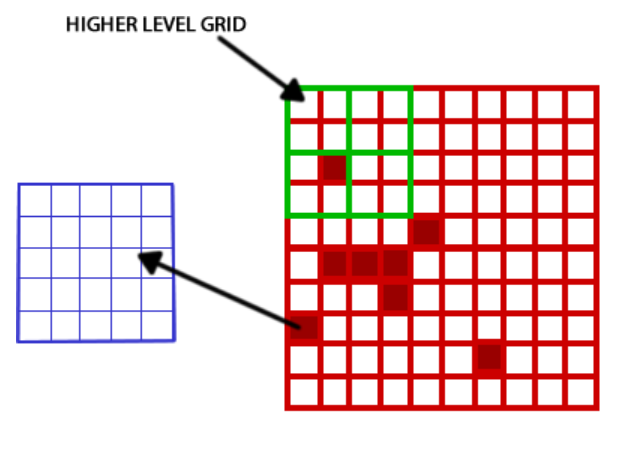
\includegraphics[width=0.9\linewidth]{figures/brickmap.png}
    \caption{Here we see the brickmap (in red), which is dense. And whenever an area in this brickmap is not homogeneous (indicated by the filled in squares), we point to a brick (in blue). \cite{van2015real}}
    \label{fig:brickmap}
\end{figure}

\noindent\textbf{Signed distance fields (SDF):} Recently, NVIDIA has done research about using SDFs to speed up traversal\cite{soderlund2022ray}. The general idea behind these distance fields is that the maximum step length a ray could take in any direction (without hitting anything) is pre-calculated, and used to skip over voxels that are known to be empty (see Figure \ref{fig:SDF_marching}). This method could be applied to most of the techniques described above, and might specifically be promising when combined with flat structures which dont implicitly store distance values by using bigger nodes in homogeneous volumes. However, calculating these SDF's is one additional step in the pipeline. Although this can be done quickly even for large volumes (less than $1$ ms for $1024^3$ voxels \cite{cao2010parallel}), it is unclear if the speedup during tracing outweighs the construction cost. Some other results from NVIDIA's paper are related to the new ray tracing graphics cards. These cards have hardware dedicated specifically to AABB and triangle intersections, and thus traversal algorithms which use these calculations can be sped up. In the paper, they did test storing bricks into a BVH, then traversing the BVH and using DDA to traverse through the bricks. Another, more interesting result they found was that storing every single voxel in a BVH actually had the fastest traversal speed. This last method makes very efficient use of the fixed function BVH traversal of the ray tracing cards, at the cost of a very large BVH.

\begin{figure}[H]
    \centering
    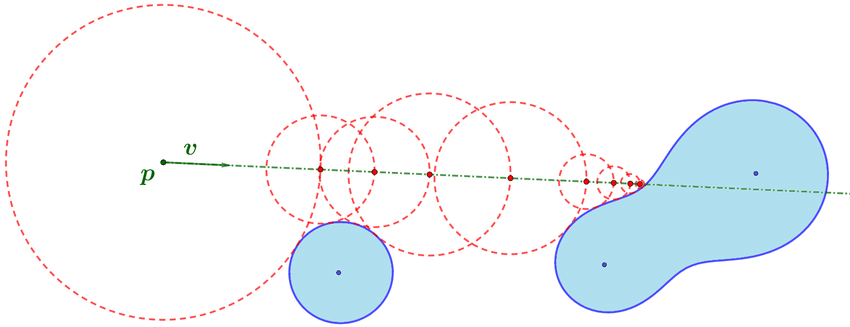
\includegraphics[width=0.9\linewidth]{figures/sdf_ray_marching.png}
    \caption{Marching through a signed distance field enables steps which are exactly as long, as the closest heterogeneity is far away. Here we see the ray in green, and the step sizes are indicated by the red circles. \cite{SDF_sphere_marching}}
    \label{fig:SDF_marching}
\end{figure}

\subsection{VDB}\label{INTRO:VDB}
In the movie industry, \textbf{VDB} \cite{museth2013vdb} has been the standard for volumetric rendering for a long time. This is a hierarchical B+tree structure with 3 layers (see Figure \ref{fig:VDB}), which optimizes for both query speed and memory size. It does so by making clever use of bitmasks, logical bitwise operations and inverted tree traversal. The last of these optimizations means that we don't have to traverse down the tree every time we query a point. But instead we assume that consecutive points will be close to each other, and remember where we are in the tree. Then the next time we query a point we start at the bottom of the tree and have $O(1)$ access time if we retrieve a point which resides in the same bottom layer. 

The VDB structure has mostly been used on the CPU. There have been implementations which port VDB to the GPU, but these do not support dynamic topology \cite{hoetzlein2016gvdb} \cite{museth2021nanovdb}. They would allow individual voxels to be modified, but can't place new voxels in arbitrary locations. This limitation makes simulation on the GPU impractical while maintaining the sparsity which makes the structure effective. The reason why this dynamic topology has never been implemented likely has to do with an inherent race condition when trying to modify any tree structure in parallel.

Research has also been conducted on encoding voxels or even internal layers of the VDB structure in neural networks \cite{kim2022neuralvdb}. These neural encodings can store a lot of detail in very limited memory, but take minutes to train. Which, again, makes dynamic updates impossible.

One very useful result of the standardization of VDB technology is the data format. Many tools can interface directly with the VDB file format \cite{VDBADeepDive}, and many artistic tools can export to the VDB file format. These features make it easy to download specific effects and test in a specific renderer.

\begin{figure}[H]
    \centering
    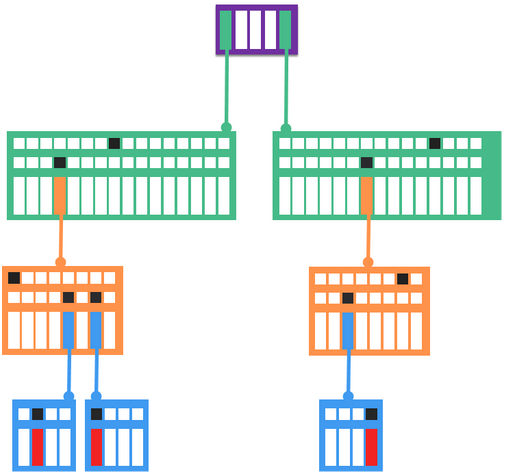
\includegraphics[width=0.9\linewidth]{figures/OpenVDB.png}
    \caption{The four level tree structure of the VDB data structure. In purple we see the top node which has arbitrary size and points to the first level of internal nodes. The two levels of internal nodes (in green and orange) both contain three rows of values. The top row is a bitmask indicating which values are "active" (this is application specific), the middle row is a bitmask indicating that a child node exists, and the bottom row containing a pointer to the child node. Then in blue we have a top row which is a bitmask indicating if a voxel is empty, and the bottom row containing the actual voxel data. \cite{museth2013vdb}}
    \label{fig:VDB}
\end{figure}

\subsection{Gaps in current research}\label{INTRO:GAPS}
To conclude the introduction we will now list the most notable issues with the current state-of-the-art, and how we can push the state-of-the-art forward in a meaningful way. Many methods have either optimized volume data structures for memory usage (ESVO, SVDAG), ray tracing performance (Brickmaps, signed distance fields) or simulation times (flat 3D array). However none of these techniques currently can do all three of these things while keeping all data and computation on the GPU. For our purposes we require an extension to the VDB data structure to enable dynamic topology on the gpu. Furthermore, combining VDB with the compression scheme of SVDAG can be explored to allow for efficient animation playback. Additionally, the combination of signed distance fields can be incorporated into the VDB structure to allow for faster ray marching through these volumes.